การออกแบบ labeling tool นั้น ผู้วิจัยได้เลือกใช้ library PyQt และภาษาไพธอนในการพัฒนา
เนื่องจาก PyQt นั้นเป็น library ที่มีผู้พัฒนาใช้กันอย่างแพร่หลาย จึงสะดวกในการศึกษา หาข้อมูลในการสร้างหรือแก้ไข
อีกทั้งยังเป็น library ที่สามารถพัฒนาด้วยภาษาไพธอนได้ และใช้งานง่าย สามารถปรับปรุงแก้ไขได้สะดวก

\subsection{แอพพลิเคชั่น labeling tool}
แอพพลิเคชั่นแบ่งการทำงานออกเป็นสี่ส่วนประกอบด้วยส่วน Select, Detect, Track และ Action label
เพื่อช่วยแบ่งเบาภาระของผู้พัฒนาในการสร้าง label สำหรับสร้างโมเดลจากข้อมูลประเภทวิดีโอ โดยส่วน Select
จะต้องสามารถตัดวิดีโอส่วนที่ไม่มีมนุษย์อยู่ออกจากวิดีโอได้ Detect ต้องสามารถหาตำแหน่งของมนุษย์ภายในวิดีโอได้
Track ต้องสามารถทำนายตำแหน่งต่อไปของมนุษย์ข้อมูลตำแหน่งของมนุษย์จาก Detect ได้
Action label ต้องสามารถทำนายการกระทำของมนุษย์ได้ในระดับหนึ่ง โดยทุกส่วนการทำงานมนุษย์ต้องสามารถทำงานร่วมกับระบบได้
ดังรูปที่ \ref{fig:labeling_overview}

\begin{figure}[!ht]
    \centering
    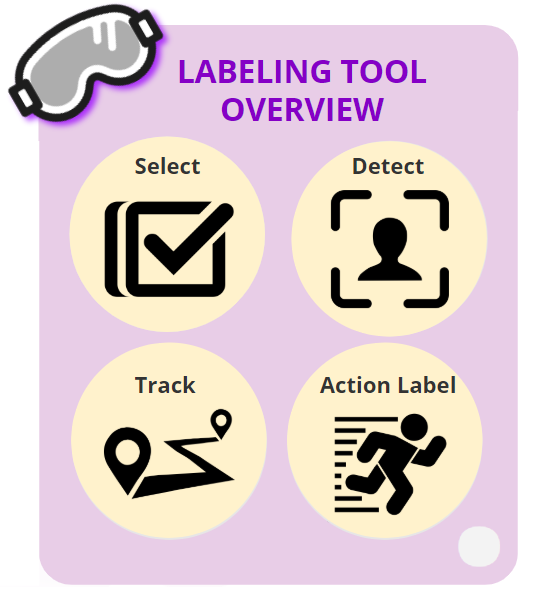
\includegraphics[width=0.7\textwidth]{chapter3/images/3_6/labelingToolOverview.png}
    \caption{ภาพรวมระบบของแอพพลิเคชั่น labeling tool}
    \label{fig:labeling_overview}
\end{figure}
\clearpage

\subsection*{โดยแต่ละส่วนจะมีรายละเอียดดังนี้}
\subsubsection{Select}
กระบวนการ Select จะต้องสามารถรับวิดีโอเข้ามา แล้วตัดวิดีโอในช่วงที่ไม่มนุษย์อยู่ในเฟรม(frame)ออกได้อัตโนมัติด้วยปัญญาประดิษฐ์
แต่เนื่องจากการประมวลผลทุกเฟรมในวิดีโอนั้นจะทำให้เสียเวลามากเกินไป จึงใช้วิธีการเลือกตัวอย่างเฟรมด้วยอัตราคงที่(สามารถกำหนดได้)
ซึ่งเรียกว่าเฟรมเหล่านี้ว่า คีย์เฟรม(keyframe) จากนั้นใช้ปัญญาประดิษฐ์ประมวลผลคีย์เฟรมที่เหล่านั้น 
เพื่อลดระยะเวลาในการประมวลผลลง และมนุษย์จะต้องสามารถแก้ไขข้อผิดพลาดของปัญญาประดิษฐ์ได้ 
เพื่อเพิ่มคุณภาพของชุดข้อมูล จึงออกแบบหน้าต่างได้ดังรูปที่ \ref{fig:SelectDraft}

\begin{figure}[!ht]
    \centering
    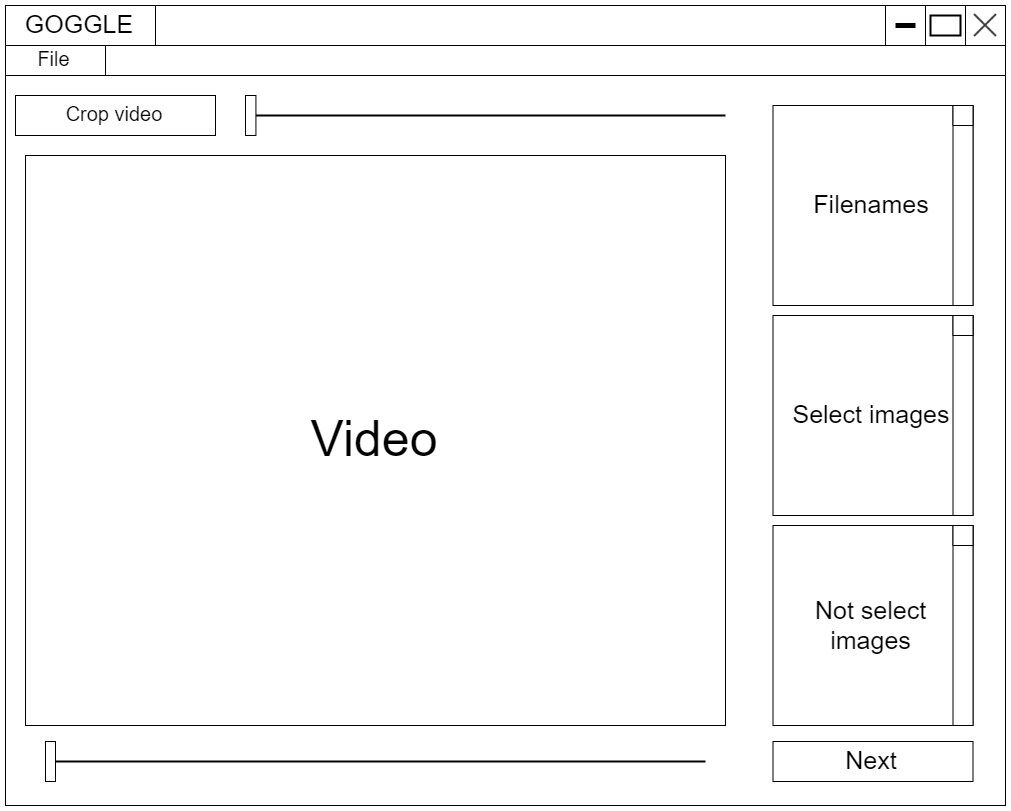
\includegraphics[width=1\textwidth]{chapter3/images/3_6/SelectDraft.png}
    \caption{หน้าต่างหน้าต่าง Select ของแอพพลิเคชั่น labeling tool}
    \label{fig:SelectDraft}
\end{figure}
\clearpage
\begin{figure}[!ht]
    \centering
    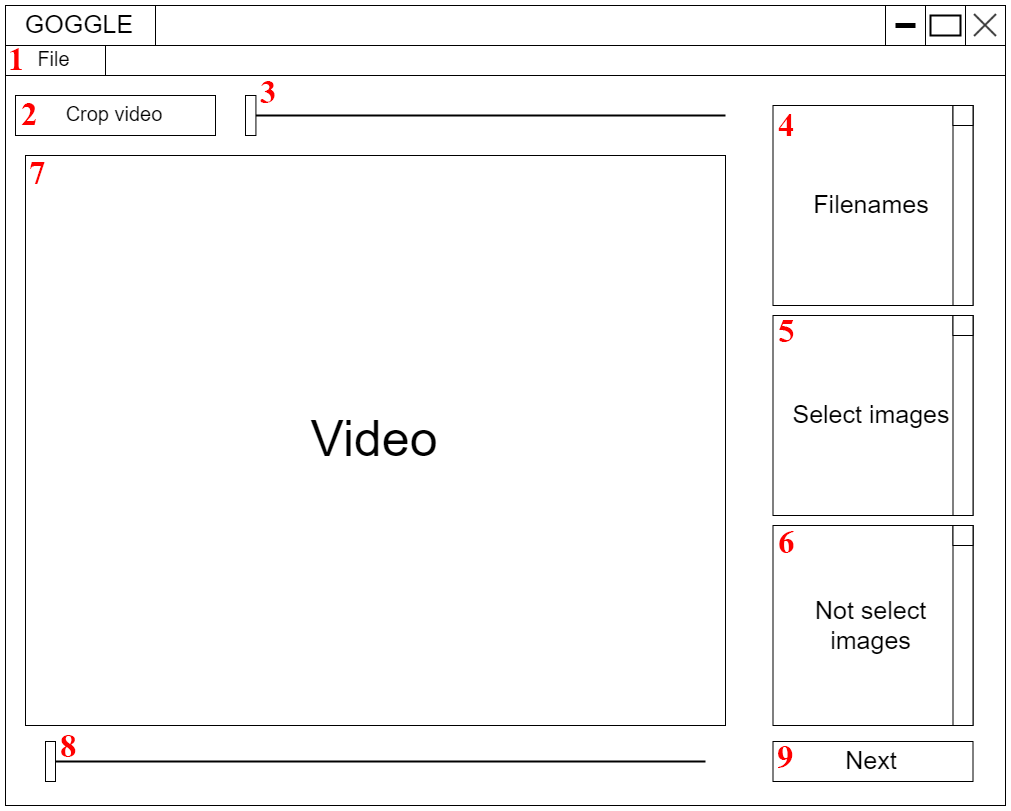
\includegraphics[width=1\textwidth]{chapter3/images/3_6/SelectDraft_point.png}
    \caption{ตำแหน่งของแต่ละวิดเจ็ตในหน้าต่าง Select}
    \label{fig:SelectDraft_point}
\end{figure}
โดยที่แต่ละวิดเจ็ตตามหมายเลขที่กำหนดตามรูปที่ \ref{fig:SelectDraft_point} มีรายละเอียดดังนี้
\begin{enumerate}
	\setlength\itemsep{-0.25em}
	\item หมายเลข 1 คือปุ่มสำหรับเลือกไฟล์วิดีโอที่ต้องการจากในคอมพิวเตอร์เข้ามาในโปรแกรม
    \item หมายเลข 2 คือปุ่มสำหรับสั่งให้ระบบทำการสร้างคีย์เฟรมขึ้นมา 
    แล้วใช้ปัญญาประดิษฐ์ประมวลผลเพื่อแยกว่าคีย์เฟรมไหนมีคนอยู่ และคีย์เฟรมไหนไม่มีคนอยู่
    แบบอัตโนมัติ(Auto mode)
    \item หมายเลข 3 คือแถบเลื่อนเพื่อกำหนดความถี่ในการหยิบคีย์เฟรม โดยจะมีช่วงอยู่ที่ 1 
    เฟรมต่อวินาที จนถึง เฟรมต่อวินาทีสูงสุดของวิดีโอที่รับเข้ามา
	\item หมายเลข 4 คือกล่องสำหรับแสดงชื่อวิดีโอที่รับเข้ามาในโปรแกรมเพื่อเลือกเข้ามาใช้ในการประมวลผล
	\item หมายเลข 5 คือกล่องสำหรับแสดงว่าคีย์เฟรมใดมีมนุษย์อยู่ในเฟรม โดยที่ผู้ใช้งานสามารถตรวจสอบความถูกต้องและแก้ไขข้อผิดพลาดของปัญญาประดิษฐ์ได้
	\item หมายเลข 6 คือกล่องสำหรับแสดงว่าคีย์เฟรมใดไม่มีมนุษย์อยู่ในเฟรม โดยที่ผู้ใช้งานสามารถตรวจสอบความถูกต้องและแก้ไขข้อผิดพลาดของปัญญาประดิษฐ์ได้
	\item หมายเลข 7 คือหน้าต่างสำหรับแสดงเฟรมที่เลือกจากหมายเลข 5 หมายเลข 6 หรือหมายเลข 8
	\item หมายเลข 8 คือแถบเลื่อนสำหรับเลื่อนดูคีย์เฟรมทั้งหมดที่ระบบสร้างขึ้น
	\item หมายเลข 9 คือปุ่มสำหรับไปกระบวนการต่อไปหลังจากระบบประมวลผลเสร็จแล้ว
\end{enumerate}
\clearpage

\subsubsection{Detect}
กระบวนการ Delect จะต้องสามารถรับคีย์เฟรมจากกระบวนการ Select มาประมวลผลด้วยปัญญาประดิษฐ์เพื่อหาตำแหน่งของมนุษย์ที่อยู่ในคีย์เฟรม 
แล้วสร้างกรอบสี่เหลี่ยมครอบบริเวณดังกล่าวได้ในแบบอัตโนมัติ เพื่อแบ่งเบาภาระผู้ใช้ในการที่ต้องสร้างกรอบสี่เหลี่ยมครอบตำแหน่งของมนุษย์ด้วยตัวเอง
และผู้ใช้ต้องสามารถสร้างหรือลบกรอบสี่เหลี่ยมได้ด้วยตัวเองสำหรับแก้ไขความผิดพลาดของปัญญาประดิษฐ์ เพื่อเพิ่มคุณภาพของชุดข้อมูล
จึงออกแบบหน้าต่างได้ดังรูปที่ \ref{fig:DetectDraft}
\begin{figure}[!ht]
    \centering
    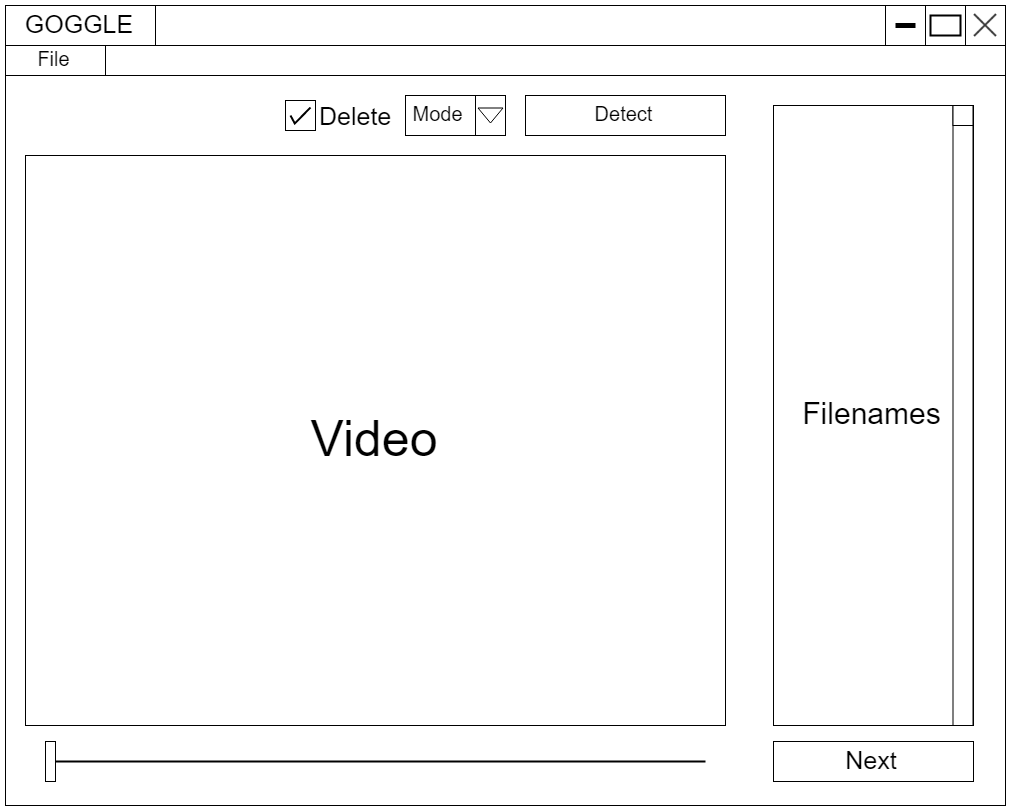
\includegraphics[width=1\textwidth]{chapter3/images/3_6/DetectDraft.png}
    \caption{หน้าต่าง Detect ของแอพพลิเคชั่น labeling tool}
    \label{fig:DetectDraft}
\end{figure}
\clearpage
\begin{figure}[!ht]
    \centering
    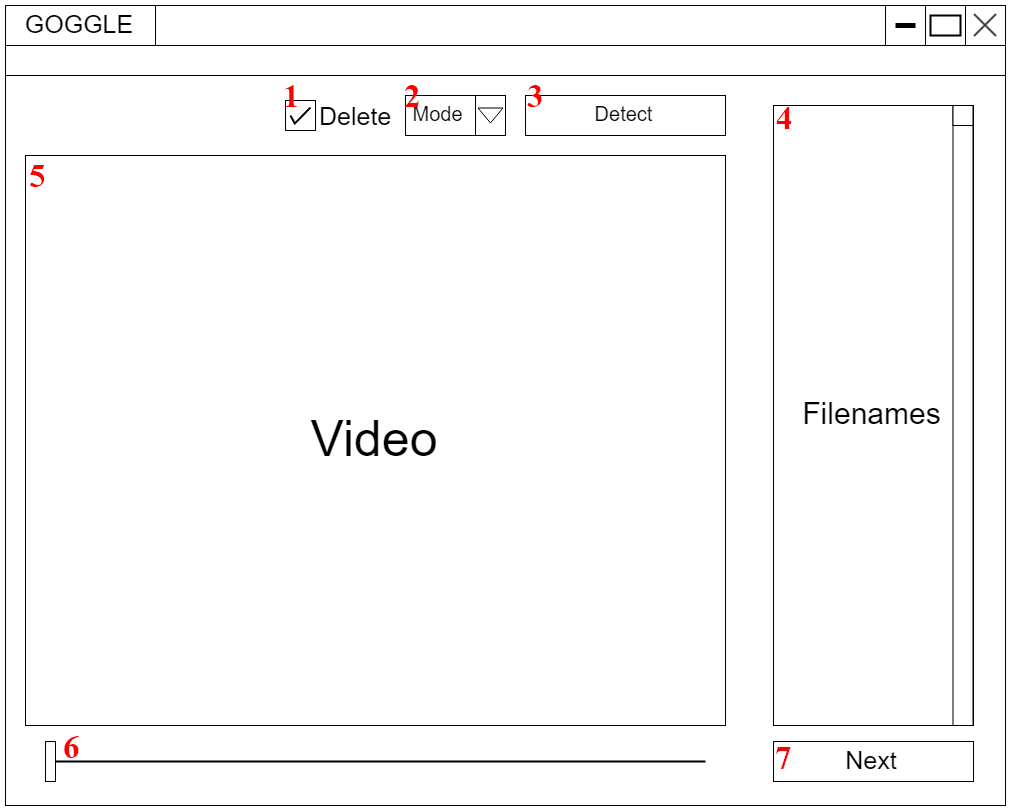
\includegraphics[width=1\textwidth]{chapter3/images/3_6/DetectDraft_point.png}
    \caption{ตำแหน่งของแต่ละวิดเจ็ตในหน้าต่าง Detect}
    \label{fig:DelectDraft_point}
\end{figure}
โดยที่แต่ละวิดเจ็ตตามหมายเลขที่กำหนดตามรูปที่ \ref{fig:DelectDraft_point} มีรายละเอียดดังนี้
\begin{enumerate}
	\setlength\itemsep{-0.25em}
    \item หมายเลข 1 คือช่องสำหรับกดเพื่อเปลี่ยนระบบจากสร้างกรอบสี่เหลี่ยมในแบบแก้ไขด้วยตนเอง(Manual mode) เป็นลบกรอบสี่เหลี่ยมแทน
    \item หมายเลข 2 คือช่องสำหรับเลือกว่าจะใช้ระบบแบบใด ระหว่างแบบอัตโนมัติและแบบแก้ไขด้วยตนเอง
    \item หมายเลข 3 คือปุ่มสำหรับสั่งให้ระบบทำการตรวจหาตำแหน่งของมนุษย์ในคีย์เฟรมทั้งหมดแล้วสร้างกรอบสี่เหลี่ยมขึ้นมาครอบบริเวณที่กำหนด
	\item หมายเลข 4 คือกล่องสำหรับแสดงคีย์เฟรมทั้งหมด
	\item หมายเลข 5 คือหน้าต่างสำหรับแสดงเฟรมที่เลือกจากหมายเลข 4 หรือหมายเลข 6
	\item หมายเลข 6 คือแถบเลื่อนสำหรับเลื่อนดูคีย์เฟรมทั้งหมดที่มี เพื่อตรวจสอบความถูกต้องของปัญญาประดิษฐ์
	\item หมายเลข 7 คือปุ่มสำหรับไปกระบวนการต่อไปหลังจากระบบประมวลผลเสร็จแล้ว
\end{enumerate}
\clearpage

\subsubsection{Track}
เนื่องจากกระบวนการ Detect นั้นจะทำเฉพาะในคีย์เฟรมทำให้ในเฟรมอื่นๆนอกเหนือจากนั้นจะไม่มีกรอบสี่เหลี่ยมอยู่
ดังนั้นกระบวนการ Track จึงต้องสามารถทำนายตำแหน่งต่อไปของมนุษย์แล้วสร้างกรอบสี่เหลี่ยมขึ้นมาบนเฟรมระหว่างคีย์เฟรมทั้งหมดได้โดยอัตโนมัติ
เพื่อสร้างข้อมูลตำแหน่งของมนุษย์ในเฟรมเหล่านั้น และผู้ใช้ต้องสามารถสร้างหรือลบกรอบสี่เหลี่ยมได้ด้วยตัวเองสำหรับแก้ไขความผิดพลาดของอัลกอริทึม
จึงออกแบบหน้าต่างได้ดังรูปที่ \ref{fig:TrackDraft}
\begin{figure}[!ht]
    \centering
    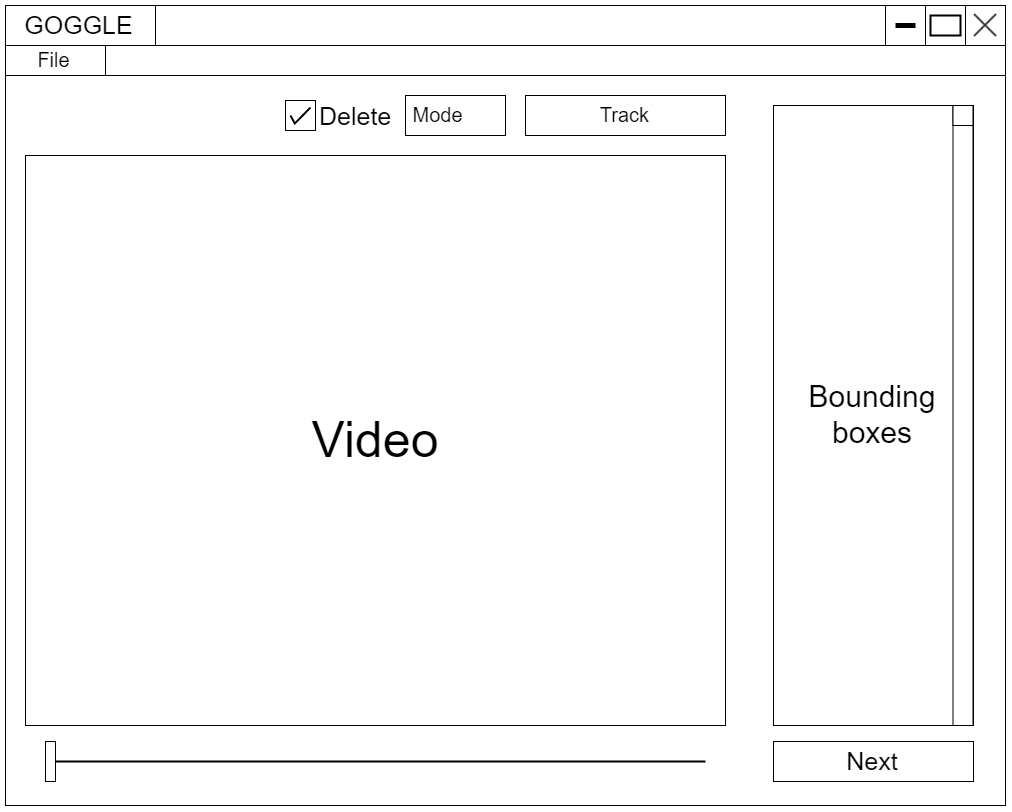
\includegraphics[width=1\textwidth]{chapter3/images/3_6/TrackDraft.png}
    \caption{หน้าต่าง Track ของแอพพลิเคชั่น labeling tool}
    \label{fig:TrackDraft}
\end{figure}
\clearpage
\begin{figure}[!ht]
    \centering
    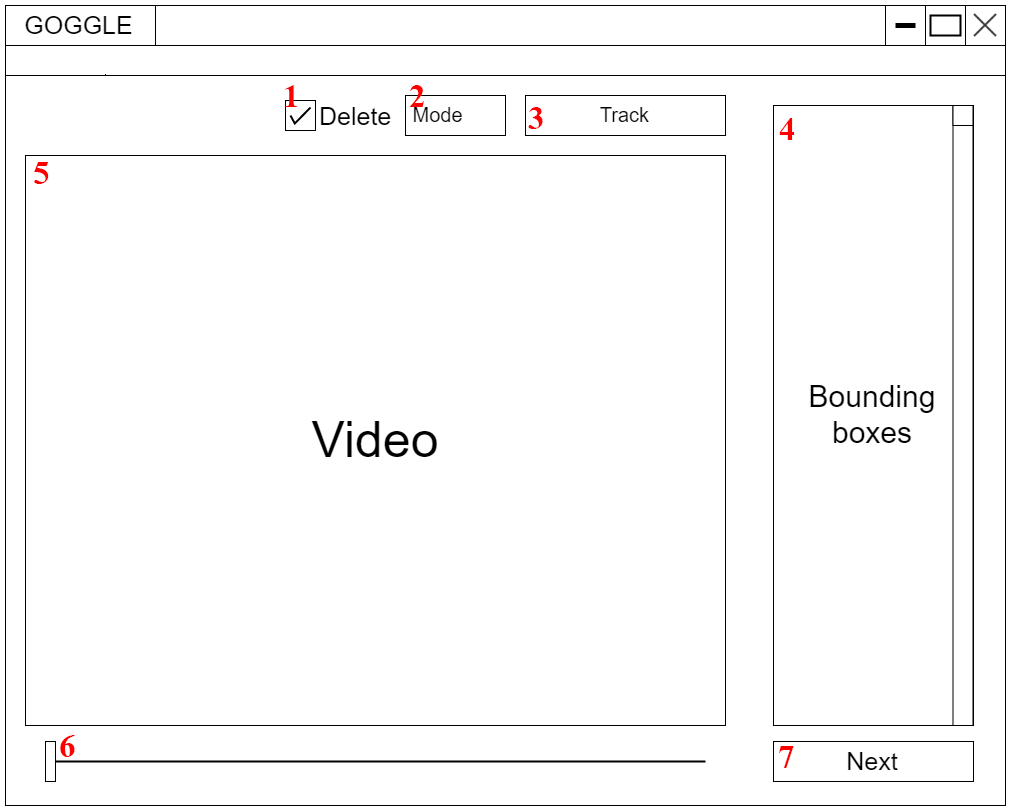
\includegraphics[width=1\textwidth]{chapter3/images/3_6/TrackDraft_point.png}
    \caption{ตำแหน่งของแต่ละวิดเจ็ตในหน้าต่าง Track}
    \label{fig:TrackDraft_point}
\end{figure}
โดยที่แต่ละวิดเจ็ตตามหมายเลขที่กำหนดตามรูปที่ \ref{fig:TrackDraft_point} มีรายละเอียดดังนี้
\begin{enumerate}
	\setlength\itemsep{-0.25em}
    \item หมายเลข 1 คือช่องสำหรับกดเพื่อเปลี่ยนระบบจากสร้างกรอบสี่เหลี่ยมในแบบแก้ไขด้วยตนเอง(Manual mode) เป็นลบกรอบสี่เหลี่ยมแทน
    \item หมายเลข 2 คือช่องสำหรับเลือกว่าจะใช้ระบบแบบใด ระหว่างแบบอัตโนมัติและแบบแก้ไขด้วยตนเอง
    \item หมายเลข 3 คือปุ่มสำหรับสั่งให้ระบบทำการตรวจหาตำแหน่งของมนุษย์ในเฟรมระหว่างคีย์เฟรมทั้งหมดแล้วสร้างกรอบสี่เหลี่ยมขึ้นมาครอบบริเวณที่กำหนด
	\item หมายเลข 4 คือกล่องสำหรับแสดงกรอบสี่เหลี่ยมทั้งหมดที่อยู่ในเฟรม
	\item หมายเลข 5 คือหน้าต่างสำหรับแสดงเฟรมที่เลือกจากหมายเลข 6
	\item หมายเลข 6 คือแถบเลื่อนสำหรับเลื่อนดูเฟรมทั้งหมดที่มี เพื่อตรวจสอบความถูกต้องของอัลกอริทึม
	\item หมายเลข 7 คือปุ่มสำหรับไปกระบวนการต่อไปหลังจากระบบประมวลผลเสร็จแล้ว
\end{enumerate}
\clearpage

\subsubsection{Action label}
กระบวนการ Action label นั้นต้องสามารถทำนายว่าการกระทำ(Action)ของมนุษย์ที่อยู่ในแต่ละเฟรมว่าคืออะไร ได้โดยอัตโนมัติด้วยปัญญาประดิษฐ์
และผู้ใช้จะต้องสามารถแก้ไขข้อผิดพลาดของปัญญาประดิษฐ์ได้หากมีการทำนายที่ผิดพลาดเกิดขึ้น
หรือถ้าหากผู้ใช้ต้องการเพิ่มการกระทำที่ไม่ได้มีอยู่ในชุดการกระทำพื้นฐานที่มีอยู่แล้วของปัญญาประดิษฐ์ ผู้ใช้ก็สามารถเพิ่มการกระทำนั้นเข้ามาได้
จึงออกแบบหน้าต่างได้ดังรูปที่ \ref{fig:ActionLabelDraft}
\begin{figure}[!ht]
    \centering
    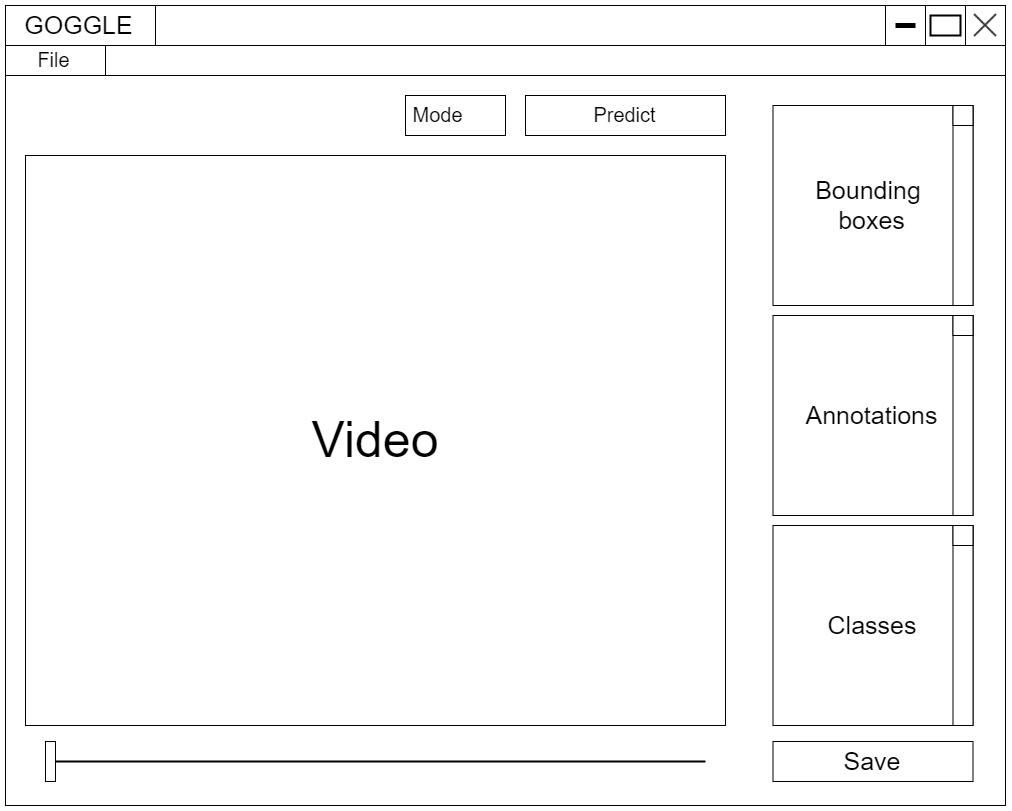
\includegraphics[width=1\textwidth]{chapter3/images/3_6/ActionLabelDraft.png}
    \caption{หน้าต่าง Action label ของแอพพลิเคชั่น labeling tool}
    \label{fig:ActionLabelDraft}
\end{figure}
\clearpage
\begin{figure}[!ht]
    \centering
    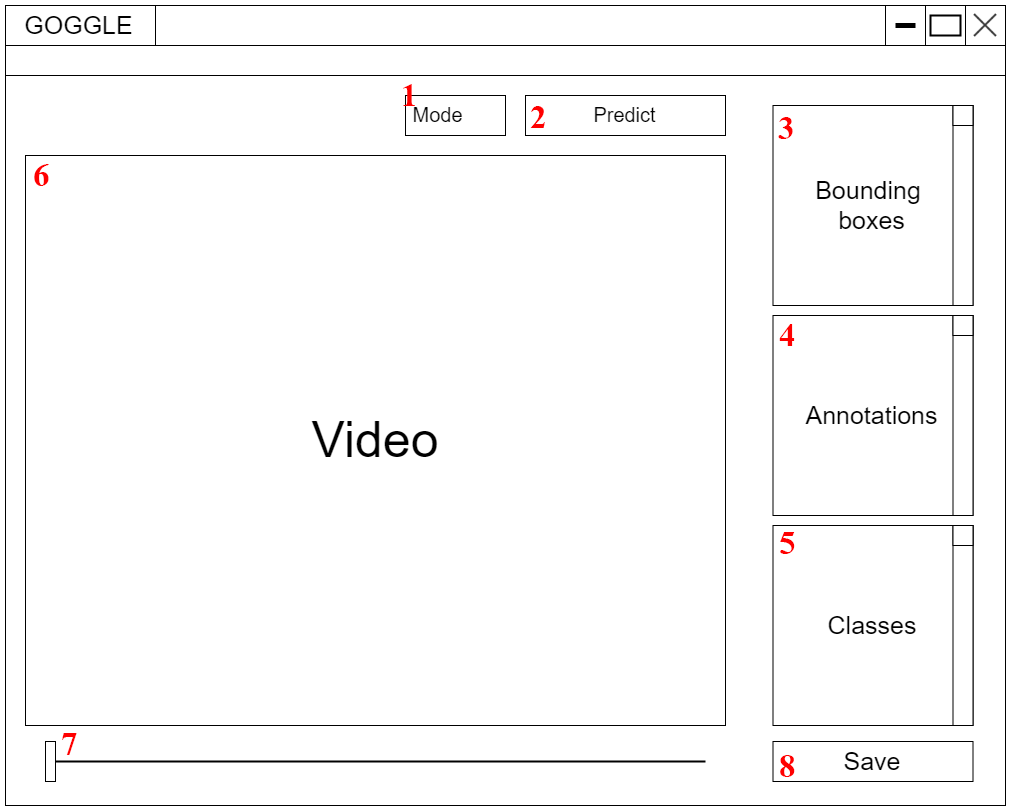
\includegraphics[width=1\textwidth]{chapter3/images/3_6/ActionLabelDraft_point.png}
    \caption{ตำแหน่งของแต่ละวิดเจ็ตในหน้าต่าง Action label}
    \label{fig:ActiobLabelDraft_point}
\end{figure}
โดยที่แต่ละวิดเจ็ตตามหมายเลขที่กำหนดตามรูปที่ \ref{fig:TrackDraft_point} มีรายละเอียดดังนี้
\begin{enumerate}
	\setlength\itemsep{-0.25em}
    \item หมายเลข 1 คือช่องสำหรับเลือกว่าจะใช้ระบบแบบใด ระหว่างแบบอัตโนมัติและแบบแก้ไขด้วยตนเอง
    \item หมายเลข 2 คือปุ่มสำหรับสั่งให้ระบบทำนายการกระทำของมนุษย์ในทุกๆเฟรม
    \item หมายเลข 3 คือกล่องสำหรับแสดงกรอบสี่เหลี่ยมทั้งหมดที่อยู่ในเฟรมที่เลือก
	\item หมายเลข 4 คือกล่องสำหรับแสดงการกระทำของมนุษย์แต่ละคนที่อยู่ในเฟรมที่เลือก โดยจะเรียงลำดับคู่กับกรอบสี่เหลี่ยมที่อยู่ในช่องหมายเลข 3
    \item หมายเลข 5 คือกล่องสำหรับแสดงชุดการกระทำที่ปัญญาประดิษฐ์มีอยู่แล้ว ซึ่งในการทำงานแบบแก้ไขด้วยตนเองนั้น จะสามารถค้นหาการกระทำที่มีอยู่แล้วได้ 
    และหากคำที่ใส่เข้ามานั้นไม่มีอยู่ในชุดการกระทำก็จะเป็นการเพิ่มการกระทำนั้นเข้ามาแทน
	\item หมายเลข 6 คือหน้าต่างสำหรับแสดงเฟรมที่เลือกจากหมายเลข 7
	\item หมายเลข 7 คือแถบเลื่อนสำหรับเลื่อนดูเฟรมทั้งหมดที่มี เพื่อตรวจสอบความถูกต้องของปัญญาประดิษฐ์
	\item หมายเลข 8 คือปุ่มสำหรับสร้างไฟล์ XML ของทุกๆเฟรมสำหรับใช้ในการสร้างโมเดลโดยรายละเอียดข้อมูลภายในไฟล์ XML จะอยู่ในหัวข้อ \ref{sec:XMLInfo}
\end{enumerate}
\clearpage

\subsubsection{รายละเอียดข้อมูลภายในไฟล์ XML}
\label{sec:XMLInfo}
ไฟล์ XML นั้นเป็นรูปแบบที่นิยมใช้ในการเก็บข้อมูลสำหรับการสร้างโมเดลประเภทตรวจจับวัตถุ(object detection)
โดยจะเก็บข้อมูลในรูปแบบของ PASCAL VOC ที่นิยมใช้ในการสร้างโมเดลด้วย library Tensorflow โดยภายในไฟล์จะมีข้อมูลดังรูปที่ \ref{fig:XMLFormat}
\begin{figure}[!ht]
    \centering
    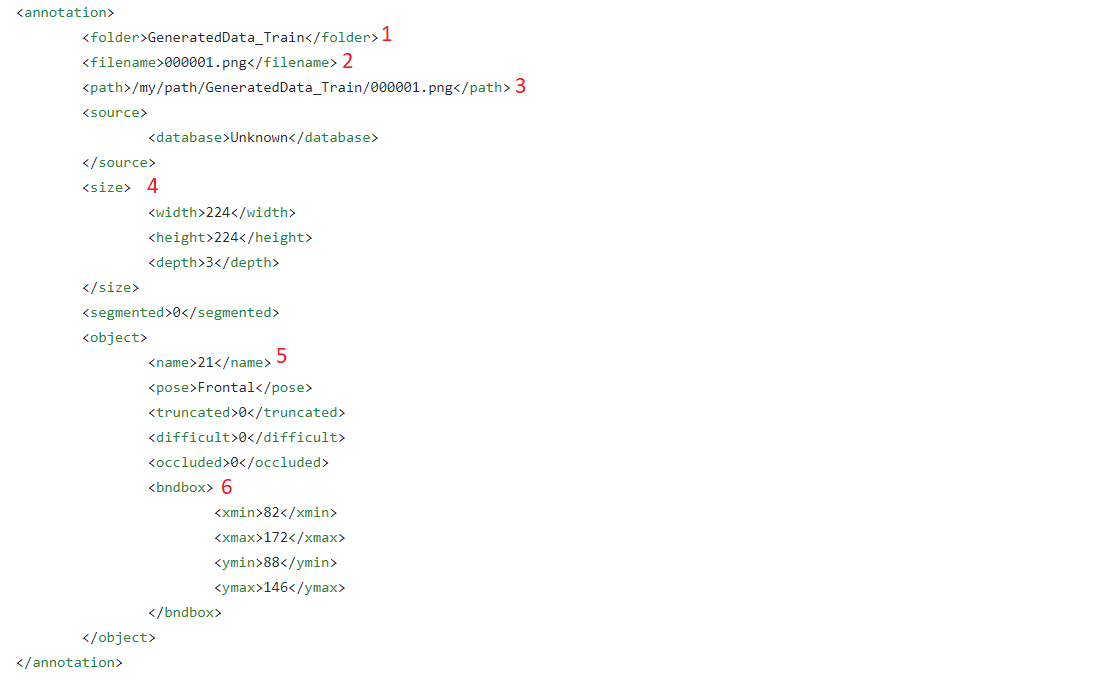
\includegraphics[width=1\textwidth]{chapter3/images/3_6/XMLFormat.png}
    \caption{ตัวอย่างข้อมูลภายในไฟล์ XML}
    \label{fig:XMLFormat}
\end{figure}
โดยข้อมูลส่วนสำคัญของรูปแบบนี้นั้นจะถูกใส่หมายเลขกำกับไว้ซึ่งแต่ละหมายเลขนั้นหมายถึง
\begin{enumerate}
	\setlength\itemsep{-0.25em}
    \item หมายเลข 1 คือชื่อโฟลเดอร์ที่เก็บไฟล์รูปภาพที่เกี่ยวข้องกับไฟล์ XML นี้อยู่
    \item หมายเลข 2 คือชื่อไฟล์ที่เกี่ยวข้องกับไฟล์ XML นี้
    \item หมายเลข 3 คือเส้นทางในคอมพิวเตอร์(directory path)ของไฟล์รูปภาพที่เกี่ยวข้องกับไฟล์ XML นี้
    \item หมายเลข 4 คือขนาดและมิติของรูปภาพ ซึ่งจะประกอบด้วยความกว้าง(wdith) ความยาว(height) และจำนวนช่องสี(depth) 
    โดยที่จำนวนช่องสีที่มีความลึก 3 มักจะหมายถึงภาพสี RGB และจำนวนช่องสีที่มีความลึก 2 จะหมายถึงภาพขาวดำ(gray scale)
	\item หมายเลข 5 คือ label ของวัตถุหรืออย่างอื่น ที่อยู่ในกรอบสี่เหลี่ยมที่ถูกกำหนดไว้ในส่วนของหมายเลข 6
	\item หมายเลข 6 คือ กรอบสี่เหลี่ยมที่ครอบวัตถุที่สนใจ เช่นมนุษย์ เป็นต้น
\end{enumerate}